\hypertarget{a00811}{}\section{Background processing callback}
\label{a00811}\index{Background processing callback@{Background processing callback}}
Background processing support for A\+AX D\+SP and Native plug-\/in algorithms. 

\hypertarget{a00811_algbgpagecontents}{}\subsection{On this page}\label{a00811_algbgpagecontents}
\begin{DoxyItemize}
\item \mbox{\hyperlink{a00811_alg_bg_desc}{Background thread description}} \item \mbox{\hyperlink{a00811_alg_bg_restrict}{Restrictions and limitations of background threads}} \item \mbox{\hyperlink{a00811_alg_bg_perf}{Background thread performance characteristics on D\+SP systems}} \item \mbox{\hyperlink{a00811_alg_bg_memmgmt}{Background thread memory management}} \item \mbox{\hyperlink{a00811_alg_bg_additionalinformation}{Additional information}}\end{DoxyItemize}
\hypertarget{a00811_alg_bg_desc}{}\subsection{Background thread description}\label{a00811_alg_bg_desc}
Each algorithm render callback may optionally be associated with a background processing callback. This background callback will be triggered regularly in an idle context on a separate thread, and can be used to perform any background task required by the algorithm.

Background thread processing is supported for both A\+AX D\+SP and A\+AX Native plug-\/ins.\hypertarget{a00811_alg_bg_restrict}{}\subsection{Restrictions and limitations of background threads}\label{a00811_alg_bg_restrict}
\begin{DoxyItemize}
\item An A\+AX D\+SP Effect that registers for background processing will not share a D\+SP with any other Effect type. It may share a D\+SP with multiple instances of its own type, but only if its resource requirements allow for this. \item The frequency of background thread executions relative to render thread executions will vary depending on the processing situation. For example, a host may pre-\/process a series of audio buffers as quickly as possible during an offline render. In this case there would be many executions of the render thread callback for each execution of the background thread callback. Be sure to consider this when using the background thread feature in plug-\/ins that support an Audio\+Suite processing type.\end{DoxyItemize}
\hypertarget{a00811_alg_bg_perf}{}\subsection{Background thread performance characteristics on D\+S\+P systems}\label{a00811_alg_bg_perf}
The background processing callback is called from a true idle thread context. On D\+SP accelerated platforms, this means that the callback will be triggered continuously whenever the chip is not executing an interrupt, i.\+e. the algorithm render callback. Since the render callback\textquotesingle{}s resource requirements are well-\/defined (or at least strictly bounded,) the background thread\textquotesingle{}s available cycles are also deterministically bounded.

However, the background thread itself has a lower priority than the D\+SP shell. While the background callback\textquotesingle{}s execution will not be interrupted by shell operations, it will be blocked in the event of a contention for memory resources with the shell. As a result, the number of memory operations that may be performed in this callback will be less well-\/defined when the host is consuming memory resources,e.\+g. when delivering a very large coefficient block to the D\+SP.

If your T\+DM plug-\/in does not perform any resource-\/intensive memory operations then you can assume a guaranteed performance level for its D\+SP background thread. Development tools are available that will test a plug-\/in by refreshing its entire context memory at every interrupt, and the background thread performance characteristics measured by these tools, plus an additional buffer to account for any pathological cases that may be missed by the performance check, should provide a guaranteed performance baseline for the background thread that will be completely safe for any Pro Tools operation scenario.\hypertarget{a00811_alg_bg_memmgmt}{}\subsection{Background thread memory management}\label{a00811_alg_bg_memmgmt}
The background processing callback is not provided with any data pointers and does not have access to any facilities for managed communication with the rest of the plug-\/in. Therefore, the background process must use shared global data structures to interact with the render callback. Your plug-\/in will need to manually synchronize access to this data.

Usually the background callback will want to interact with the render callback via the algorithm\textquotesingle{}s private data blocks. Therefore, private data blocks that are provided to an algorithm\textquotesingle{}s context will not be relocated by the host between calls to the render callback, and background processes can reliably access this data once provided with a pointer. The same is not true for audio buffers, meters, coefficient ports, etc. -\/ this data can all be relocated by the host when the render callback is not executing.\hypertarget{a00811_alg_bg_additionalinformation}{}\subsection{Additional information}\label{a00811_alg_bg_additionalinformation}
{\bfseries{TI Guide}} \begin{DoxyItemize}
\item \mbox{\hyperlink{a00832_subsubsection__background_processing_}{Background processing}} \item \mbox{\hyperlink{a00832_subsubsection__dma_and_background_thread_performance_reporting_}{D\+MA and background thread performance reporting}} \end{DoxyItemize}
Collaboration diagram for Background processing callback\+:
\nopagebreak
\begin{figure}[H]
\begin{center}
\leavevmode
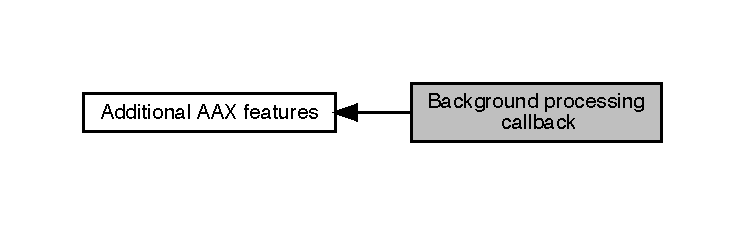
\includegraphics[width=350pt]{a00811}
\end{center}
\end{figure}
